%% DONE
\id{МРНТИ 65.63.29}{https://doi.org/10.58805/kazutb.v.1.26-761}

\begin{articleheader}
\sectionwithauthors{Д.С. Свидерская, Е.Ф. Краснопёрова, А.М. Шуленова, Н.Е. Камзина}{ИССЛЕДОВАНИЕ КАЧЕСТВЕННЫХ ПОКАЗАТЕЛЕЙ МОРОЖЕНОГО ПРИ ИСПОЛЬЗОВАНИИ ПЛОДОВО-ЯГОДНОГО НАПОЛНИТЕЛЯ}

{\bfseries
\textsuperscript{1}Д.С. Свидерская\textsuperscript{\envelope } \alink{https://orcid.org/0000-0003-3329-1126},
\textsuperscript{2}Е.Ф. Краснопёрова\alink{https://orcid.org/0000-0002-9336-0026},
\textsuperscript{1}Н.Е. Камзина\alink{https://orcid.org/0000-0002-2482-2645},
\textsuperscript{3}А.М. Шуленова\alink{https://orcid.org/0009-0003-2812-075X}}
\end{articleheader}

\begin{affiliation}
\emph{\textsuperscript{1}Торайгыров университет, Павлодар, Казахстан,}

\emph{\textsuperscript{2}Инновационный Евразийский университет, Павлодар, Казахстан,}

\emph{\textsuperscript{3}Казахский агротехнический исследовательский университет им. Сакена Сейфуллина, Астана, Казахстан}

\raggedright \textsuperscript{\envelope }{\em Корреспондент-автор: \href{mailto:sofilsev@rambler.ru}{\nolinkurl{sofilsev@rambler.ru}}}
\end{affiliation}

Статья посвящена перспективам использования дикорастущих плодов и ягод,
таких как ирга, черемуха и рябина красная, в производстве продуктов
переработки молока. Выбранное растительное сырье характеризуется:
высоким содержанием пектиновых веществ, обладающих радиопротекторными
свойствами, благодаря которым готовые изделия могут быть рекомендованы
для экологически неблагоприятных регионов с загрязненными воздухом,
водой и почвой вредными и опасными веществами; антибактериальными
свойствами, препятствующими развитию инфекционных заболеваний, подавляя
развитие вредных микроорганизмов; большим количеством витаминов,
оказывающим общеукрепляющих эффект на организм человека.

Представлены результаты исследований влияния разработанной добавки
растительного происхождения на такие важные качественные показатели
молочного продукта -- мороженого, как органолептические (запах и вкус,
структура и консистенция, цвет), физико-химические (содержание молочного
жира, сахарозы, сухих веществ и кислотность) и микробиологические
(бактерии группы кишечных палочек, St. Aureus, патогенные
микроорганизмы). Опираясь на представленные данные, определено
оптимальное количество вносимой добавки из ягод ирги и плодов черемухи и
рябины красной. Эти же показатели были определены в готовом молочном
продукте, результаты которых свидетельствуют о соответствии мороженого
требованиям, изложенным в действующей нормативно-технической
документации.

Акцентировано внимание на необходимости создания продуктов, обогащенных
натуральными природными компонентами, которые способны заменить
искусственные добавки и часть дорогостоящего молочного сырья, не снижая
качественных характеристик готовой продукции. Показано, что молочное
сырье наилучшим образом сочетается с сырьем растительного происхождения,
что дает возможность производства целой продуктовой линейки.

{\bfseries Ключевые слова}: мороженое, растительная добавка, черемуха,
ирга, рябина красная.

\begin{articleheader}
{\bfseries ЖЕМІС-ЖИДЕК ТОЛТЫРҒЫШЫН ПАЙДАЛАНУ КЕЗІНДЕ БАЛМҰЗДАҚТЫҢ САПАЛЫҚ КӨРСЕТКІШТЕРІН ЗЕРТТЕУ}

{\bfseries
\textsuperscript{1}Д.С. Свидерская\textsuperscript{\envelope },
\textsuperscript{2}Е.Ф. Краснопёрова,
\textsuperscript{1}Н.Е. Қамзина,
\textsuperscript{3}А.М. Шуленова}
\end{articleheader}

\begin{affiliation}
\emph{\textsuperscript{1}Торайғыров университеті, Павлодар, Қазақстан,}

\emph{\textsuperscript{2}Инновациялық Еуразия университеті, Павлодар, Қазақстан,}

\emph{\textsuperscript{3}Сәкен Сейфуллин атындағы Қазақ агротехникалық зерттеу университеті, Астана, Қазақстан,}

\emph{e-mail: \href{mailto:sofilsev@rambler.ru}{\nolinkurl{sofilsev@rambler.ru}}}
\end{affiliation}

Мақала сүт өңдеу өнімдерін өндіруде сервистік жидек, шие және қызыл
шетен сияқты жабайы жемістер мен жидектерді пайдалану перспективаларына
арналған. Таңдалған өсімдік шикізаты мыналармен сипатталады:
радиопротекторлық қасиеттері бар пектиндік заттардың жоғары мөлшері,
соның арқасында дайын өнімдерді ауамен, сумен және топырақпен ластанған
зиянды және қауіпті заттары бар. Экологиялық қолайсыз аймақтарға ұсынуға
болады; зиянды микроорганизмдердің дамуын тежейтін жұқпалы аурулардың
дамуына кедергі келтіретін. Бактерияға қарсы қасиеттері; адам ағзасына
жалпы күшейтетін әсері бар көптеген дәрумендер.

Әзірленген өсімдік тектес қоспаның сүт өнімі -- балмұздақтың
органолептикалық (иісі мен дәмі, құрылымы мен консистенциясы, түсі),
физика-химиялық (сүт майы, сахароза, қатты заттар мен қышқылдық құрамы)
және микробиологиялық (ішек таяқшалары тобының бактериялары, St. Aureus,
патогендік микроорганизмдер). Ұсынылған мәліметтерге сүйене отырып, ирги
жидектері мен құс шие мен қызыл тау күлінің жемістерінен алынған
қоспаның оңтайлы мөлшері анықталды. Дәл осы көрсеткіштер дайын сүт
өнімінде анықталды, олардың нәтижелері балмұздақтың қолданыстағы\\
нормативтік-техникалық құжаттамада көрсетілген талаптарға сәйкестігін
көрсетеді.

Дайын өнімнің сапалық сипаттамаларын төмендетпей, жасанды қоспалар мен
қымбат сүт шикізатының бір бөлігін алмастыра алатын табиғи
компоненттермен байытылған өнімдерді жасау қажеттілігіне баса назар
аударылады. Сүт шикізаты өсімдік тектес шикізатпен жақсы үйлесетіні
көрсетілген, бұл бүкіл өнім желісін өндіруге мүмкіндік береді.

{\bfseries Түйін сөздер:} балмұздақ, өсімдік қоспасы, құс шие, ирга, қызыл
шетен.

\begin{articleheader}
{\bfseries RESEARCH OF QUALITATIVE INDICATORS OF ICE CREAM USING FRUIT AND BERRY FILLING}

{\bfseries
\textsuperscript{1}D.Sviderskaya\textsuperscript{\envelope },
\textsuperscript{2}E.Krasnopyorova
\textsuperscript{1}N.Kamzina,
\textsuperscript{3}A.Shulenova}
\end{articleheader}

\begin{affiliation}
\emph{\textsuperscript{1}Toraigyrov University, Pavlodar, Kazakhstan,}

\emph{\textsuperscript{2}Innovative University of Eurasia, Pavlodar, Kazakhstan,}

\emph{\textsuperscript{3}Saken Seifullin Kazakh Agrotechnical Research University, Astana, Kazakhstan,}

\emph{e-mail: \href{mailto:sofilsev@rambler.ru}{\nolinkurl{sofilsev@rambler.ru}}}
\end{affiliation}

The article is devoted to the prospects for the use of wild fruits and
berries, such as irga, bird cherry and red mountain ash, in the
production of milk processing products. Selected plant raw materials are
characterized by: a high content of pectin substances with
radioprotective properties, due to which finished products can be
recommended for environmentally unfavorable regions with harmful and
hazardous \\substances contaminated with air, water and soil;
antibacterial properties that prevent the development of infectious
diseases, inhibiting the development of harmful microorganisms; a large
amount of vitamins, which has a general strengthening effect on the
human body.

The results of studies of the effect of the developed additive of plant
origin on such important qualitative indicators of the dairy product -
ice cream, as organoleptic (smell and taste, structure and consistency,
color), physicochemical (content of milk fat, sucrose, solids and
acidity) and microbiological (bacteria of the Escherichia coli group,
St. Aureus, pathogens) are presented. Based on the presented data, the
optimal amount of added additive from irga berries and fruits of bird
cherry and red mountain ash was determined. The same indicators were
determined in the finished dairy product, the results of which indicate
that the ice cream meets the requirements set forth in the current
regulatory and technical documentation.

Attention is focused on the need to create products enriched with
natural components that can replace artificial additives and part of
expensive dairy raw materials without reducing the quality
characteristics of the finished product. It has been shown that milk raw
materials are best combined with raw materials of plant origin, which
makes it possible to produce a whole product line.

{\bfseries Keywords:} ice cream, vegetable additive, bird cherry, irga,
mountain ash red

\begin{multicols}{2}
{\bfseries Введение.} Несколько десятилетий отечественные и зарубежные
ученые бьют тревогу о состоянии окружающей среды, которая имеет
тенденцию постоянного ухудшения {[}1{]}. Проявляется это в загрязнении
воздуха от постоянных выбросов производственных гигантов не смотря на
использование очистных сооружений; в загрязнении водных ресурсов из-за
сброса сточных вод; в загрязнении почвы при добыче природных ископаемых
{[}2{]}.

Также существенное влияние на окружающую среду имеют различные виды
транспорта, количество которого постоянно возрастает {[}3{]}. Не
проходят бесследно аварийные ситуации, не редко возникающие на
предприятиях. Кроме того, отрицательное влияние оказывают природные
катастрофы, например масштабное наводнение {[}4{]}.

Все это в совокупности оказывает негативное влияние на состояние
здоровья человека. Большое количество вредных веществ поступает в наш
организм через органы дыхания и с продуктами животного и растительного
происхождения, сырье для которых выращивается в таких же условиях.

Конечно, природа имеет способность к самоочищению, но живому организму
нужен воздух, вода и продукты питания здесь и сейчас. И вероятно,
найдутся и те, кто скажет, что современные технологии позволяют
сократить и контролировать объем выбросов в атмосферу. Но этого
недостаточно и убедиться в этом можно в зимний период, когда наблюдаем
за снегом, который имеет не характерный серый или розоватый оттенок. Так
же нам могут объяснять, что вода, необходимая для питьевых нужд проходит
множество ступеней очистки. А в результате мы получаем, как говориться
«мертвую» воду, лишенную всего природного и полезного для человека. Что
касается сырья, применяемого при производстве продуктов различных
пищевых отраслей, то оно конечно должно подвергаться жесткому контролю
на соответствие установленным предельным концентрациям вредных веществ.
Такому же контролю подвергаются и готовые продукты питания. Однако
требования контролируют каждое сырье или каждый продукт в отдельности.
При этом мало кто задумывается о том, какое количество вредных веществ
поступает в организм в совокупности потребления различных продуктов в
течении суток.

Принимая во внимание существующую ситуацию, целью работы являлось
создание таких продуктов питания, которые способны оказать
поддерживающий, укрепляющий и оздоравливающий эффект организму человека
на разных этапах развития, начиная с раннего детского возраста. Ко всему
этому, важно отказаться от компонентов искусственного происхождения,
вносимых для стабилизации консистенции устойчивости окраски, увеличения
срока хранения, а также способные придать нужный цвет, вкус и аромат
{[}5{]}.

Выбор следует делать в пользу ингредиентов растительного происхождения,
которые могут полноценно выполнить задачу по формированию
органолептически привлекательных пищевых продуктов. И, что самое
главное, обогатить их полезными природными веществами, придающими
готовому продукту действия направленного характера.

В процессе проведения исследований наше внимание привлекли плоды и ягоды
дикорастущие такие как ирга колосистая, черемуха обыкновенная и рябина
обыкновенная (красная), которым еще недостаточно уделяется внимания и
которые крайне редко используются отечественными производителями.
Результаты работ многих ученых дают возможность в полной мере изучить
состав таких дикоросов и оценить их свойства, оказывающие положительный
эффект на организм человека {[}6-11{]}.

Ранее нами были представлены результаты изучения совместного применения
отмеченных плодов и ягод в сочетании наиболее приемлемом для молочных
продуктов. Из всех свойств ирги, черемухи и рябины особое внимание
следует уделить содержанию пектиновых веществ, антоцианов и
антибактериальным свойствам. Пектиновые вещества можно назвать природным
сорбентом, который обладает способностью образовывать в организме
человека стойкие комплексы с тяжелыми металлами (кадмий, свинец. ртуть,
мышьяк, цинк, медь) и радионуклидами. Такие комплексы не допускают
всасывания в кровь вредных веществ и выводят их из организма. Антоцианы
проявляют терапевтический эффект при онкологических и
сердечно-сосудистых заболеваниях. Антибактериальные свойства проявляются
за счет содержания сорбиновой кислоты, которая помогают справиться с
инфекционными заболеваниями, обладает ингибирующими и антиокислительными
свойствами, замедляя процесс распада белка и окисления липидов.
Благодаря этому возможно сокращения искусственных консервантов, широко
используемых в пищевой промышленности.

Новизна данного исследования заключается в том, что впервые подобрано
гармоничное сочетание дикорастущих плодов и ягод, в качестве добавки
растительного происхождения, благоприятно влияющего на качественные
показатели такого молочного продукта как мороженое, придавая ему
комплекс свойств направленного действия.

{\bfseries Материалы и методы.} Объектом исследований, по созданию
молочного продукта, отвечающего современным требованиям, является
мороженое. Это одно из популярнейших лакомств среди детей и взрослых.
Продукт, который хорошо «принимает» различные наполнители, позволяя
разработать широчайший ассортимент, способный удовлетворить предпочтения
самого привередливого потребителя.

Исследования по определению процентного содержания вносимой добавки и ее
влияния на качественные характеристики молочного продукта, проводились
на кафедре «Инженерия и промышленные технологии» Инновационного
Евразийского университета города Павлодар.

В качестве добавки растительного происхождения было решено использовать
ранее упомянутые дикорастущие плоды и ягоды в высушенном и измельченном
до состояния муки виде, оптимальное соотношение которых составляет 1:2:1
соответственно ирги колосистой, черемухи обыкновенной и рябины
обыкновенной (красной).

При этом, исследовались органолептические и физико-химические
показатели, характеризующие качество готового продукта, в образцах с
различным содержанием растительной добавки в сравнении с контрольным
образцом, изготовленным по традиционной технологии без наполнителей. При
этом использовались стандартизированные методики исследований,
изложенные в следующей нормативной документации: Определение
органолептических показателей проводили в соответствии с СТ РК 1732-2007
- Молоко и молочные продукты. Органолептический метод определения
показателей качества {[}12{]}; ГОСТ 3626 -73 - Молоко и молочные
продукты. Методы определения влаги и сухого вещества {[}13{]}; СТ РК ИСО
8262-2-2009 Продукты молочные и пищевые продукты на основе молока.
Определение содержания жира гравиметрическим методом Вейбулла-Бернтропа
(контрольный метод). Часть 2. Мороженое и смеси для мороженого {[}14{]};
ГОСТ 31085- 2002 - Молоко и молочные продукты. Метод определения
сахарозы и глюкозы {[}15{]}; ГОСТ ISO 8069-2013 - Молоко сухое.
Определение содержания молочной кислоты и лактатов {[}16{]}; ГОСТ
9225-84 - Молоко и молочные продукты. Методы микробиологического анализа
{[}17{]}.

{\bfseries Результаты и обсуждение.} Для этого первоначально исследовано
влияние различного количества добавки на органолептические показатели
мороженого. В подготовленные образцы вносили 5, 10, 15, 20, 25, 30 \%
добавки (таблица 1).

Установлено, что по таким характеристикам как: запах и вкус, структура и
консистенция, цвет, исследуемый продукт соответствует требованиям,
изложенным в СТ РК 1733-2015 - Молоко и молочные продукты. Общие
технические условия {[}18{]}.

По результатам исследования органолептических показателей продукции,
представленных в таблице 1, определен лучший образец продукта с
внесением добавки 20 \%. Увеличение содержания порошка из сушеных плодов
и ягод приводит к появлению привкуса остроты, которую дает рябина;
становится явно заметны частицы добавки; цвет становится неприятным
из-за сизого оттенка от ягод ирги.

Далее исследовалось изменение ряда физико-химических показателей, в
зависимости от количества вносимой растительной добавки (содержания
сухих веществ, молочного жира, сахарозы и кислотность).

Содержание сухих веществ (рисунок 1) определяли до созревания смеси
продукта и после.
\end{multicols}

\begin{table}[H]
\caption*{Таблица 1 - Результаты исследования органолептических показателей продукции}
\centering
\begin{tblr}{
  colspec = {X[0.5] X[2] X[1] X[1]},
  cells = {c},
  cell{1}{1} = {r=2}{},
  cell{1}{2} = {c=3}{},
  vlines,
  hlines,
}
Добавка, \% & Показатель, балл                                                                       &                                    &                                     \\
            & Запах и вкус,                                                                          & Структура и консистенция           & Цвет                                \\
5           & чистый                                                                                 & однородная                         & молочный                            \\
10          & чистый                                                                                 & однородная                         & молочный                            \\
15          & молочный, с едва заметным миндально-ореховым ароматом                                  & однородная                         & молочно- кремовый                   \\
20          & молочный, с легким миндально-фруктовым ароматом и привкусом                            & с едва заметными частицами добавки & кремово коричневый                  \\
25          & молочный, с выраженным миндально-фруктовым ароматом и несвойственным привкусом остроты & с наличием частиц добавки          & кремово коричневый с сизым оттенком \\
30          & молочный, с ярким миндально-фруктовым ароматом и несвойственным горьковатым привкусом  & с явными частиц добавки            & коричневый с буро-сизым оттенком    
\end{tblr}
\end{table}

\begin{figure}[H]
	\centering
	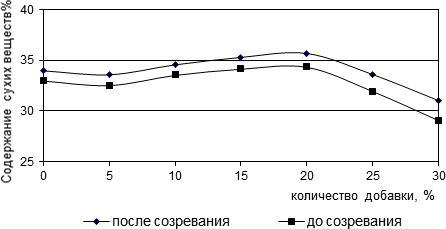
\includegraphics[width=0.6\textwidth]{media/pish2/image10}
	\caption*{Рис. 1 - Изменения содержания сухих веществ от количества добавки}
\end{figure}

\begin{multicols}{2}
Данные, представленные на рисунке 1 свидетельствуют об увеличении
содержания сухих веществ при процентном увеличении растительной добавки
до 20 \%, что объясняется высоким содержанием сухих веществ в самой
добавке, и приводит к повышению общей массовой доли сухих веществ. Так
же их увеличение связано с тем, что при созревании повышается вязкость
из-за гидратации белка и стабилизатора. Данный показатель подтверждает
наличие пектина в используемых плодах и ягодах, который обладает
вяжущими свойствами и способен сократить количество применяемого
стабилизатора.

Но при внесении добавки в количестве 25 и 30 \% наблюдается уменьшение
данного показателя, что объясняется существенным понижением сахарозы в
опытных образцах. Уменьшение количества сахарозы связано с заменой части
молочной смеси мороженого на растительную добавку.

Далее определяли содержание молочного жира, важность которого связана с
его влиянием на вкусовые характеристики готового продукта и состояние
консистенции, а также на пищевую ценность и усвояемость (рисунок 2).
\end{multicols}

\begin{figure}[H]
	\centering
	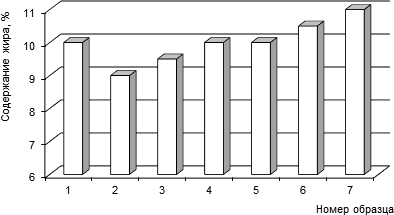
\includegraphics[width=0.6\textwidth]{media/pish2/image11}
	\caption*{\normalfont 1 - без добавки; 2 - 5 \%; 3 - 10 \%; 4 - 15 \%; 5 - 20 \%; 6 - 25 \%; 7 - 30 \%}
	\caption*{Рис. 2 - Изменение содержания молочного жира от количества добавки}
\end{figure}

\begin{multicols}{2}
На рисунке 2 представлены результаты исследований свидетельствующие, что
массовая доля жира в опытных образцах составила: при 5 \%-ом внесении
растительной добавки - 9 \%; при 10 \%-ом -- 9,5 \%; при 15 \%-ом --
10,0 \%; при 20 \%-ом -- 10,0 \%; при 25 \%-ом -- 10,5 \% и при 30 \%-ом
-- 11,0 \%.

Сохранение в молочном продукте, содержащем растительную добавку, нежного
молочного привкуса, необходимо было при увеличении количества добавки,
увеличивать количество жиросодержащего молочного сырья в опытных
образцах смеси мороженого.

Определение содержания сахарозы (рисунок 3), необходимо в связи с тем,
что она действует как подслащивающее вещество, снижает точку замерзания
и влияет на консистенцию готового продукта.
\end{multicols}

\begin{figure}[H]
	\centering
	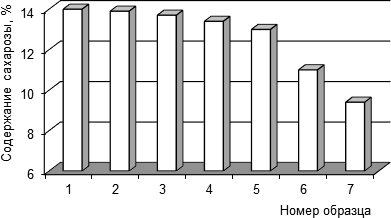
\includegraphics[width=0.6\textwidth]{media/pish2/image12}
	\caption*{1 - без добавки; 2 - 5 \%; 3 -10 \%; 4 - 15 \%; 5 - 20 \%; 6 - 25 \%; 7 - 30 \%}
	\caption*{Рис. 3 - Изменение содержания сахарозы от количества добавки}
\end{figure}

\begin{multicols}{2}
Результаты рисунка 3 указывают на снижение сахарозы при увеличении
количества вносимой добавки. Особенно резкое понижение наблюдается с
5-го образца, но как показывают органолептические показатели, снижения
сладости во вкусе не выявлено. Это объясняется наличием в ягодах ирги
сахарозы и глюкозы. Кроме того, этот факт можно рассматривать как
положительный момент, благодаря которому возможно уменьшение
производственного расхода сахара.

Следующим показателем, подвергнутым исследованию, является кислотность
(рисунок 4).
\end{multicols}

\begin{figure}[H]
	\centering
	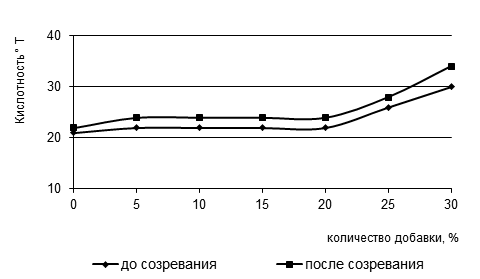
\includegraphics[width=0.6\textwidth]{media/pish2/image13}
	\caption*{Рис. 4 - Изменения кислотности от количества добавки}
\end{figure}

\begin{table}[H]
\caption*{Таблица 2 - Расчет рецептуры нового продукта}
\centering
\begin{tblr}{
  colspec = {X[2] X[1] X[1] X[1]},
  row{2} = {c},
  cell{1}{1} = {r=2}{},
  cell{1}{2} = {c=3}{c},
  cell{3}{2} = {c},
  cell{3}{3} = {c},
  cell{3}{4} = {c},
  cell{4}{2} = {c},
  cell{4}{3} = {c},
  cell{4}{4} = {c},
  cell{5}{2} = {c},
  cell{5}{3} = {c},
  cell{5}{4} = {c},
  cell{6}{2} = {c},
  cell{6}{3} = {c},
  cell{6}{4} = {c},
  cell{7}{2} = {c},
  cell{7}{3} = {c},
  cell{7}{4} = {c},
  cell{8}{2} = {c},
  cell{8}{3} = {c},
  cell{8}{4} = {c},
  cell{9}{2} = {c},
  cell{9}{3} = {c},
  cell{9}{4} = {c},
  cell{10}{2} = {c},
  cell{10}{3} = {c},
  cell{10}{4} = {c},
  vlines,
  hlines,
}
Ингредиенты                                        & Мороженое &           &         \\
                                                   & молочное  & сливочное & пломбир \\
Молоко коровье цельное(жир 3,2 \%; СОМО 8,1 \%)    & 600       & 500       & 200     \\
Сливки из коровьего молока(жир 40 \%; СОМО 4,8 \%) & 39,5      & 160       & 359     \\
Молоко коровье сухое обезжиренное(СОМО 93 \%)      & 8,1       & 10,6      & 26,4    \\
Сахар песок                                        & 130       & 120       & 120     \\
Порошок из сухих плодов и ягод                     & 200       & 200       & 200     \\
Стабилизатор                                       & 2,5       & 2,5       & 2,5     \\
Вода питьевая                                      & 19,9      & 6,9       & 92,1    \\
Итого                                              & 1000      & 1000      & 1000    
\end{tblr}
\end{table}

\begin{multicols}{2}
По результатам исследования кислотности, представленным на рисунке 4,
выявлено ее увеличение начиная с образца с количеством добавки 25 \%.
Происходит это из-за наличия в плодах и ягодах органических кислот.

Также наблюдается увеличение кислотности после созревания смеси
продукта. Так при внесении добавки от 5 до 25 \% показатель возрос на 2
°Т, хотя негативного влияния на вкусовые свойства не наблюдалось. Но при
использовании добавки в количестве 30 \% кислотность возросла на 4 °Т и
это отразилось на вкусовом восприятии в сторону ухудшения.

В результате исследованных органолептических и основных, для мороженого,
физико-химических показателей лучшим вариантом выбран опытный образец
продукта с внесением добавки в количестве 20 \% и рассчитана рецептура
нового продукта (таблица 2).

Производство опытной партии нового продукта осуществлено в соответствии
с традиционной технологией при использовании оборудования, которым
оснащены современные предприятия молочной промышленности.

На заключительном этапе данной работы проведено определение
органолептических показателей готового продукта -- мороженого (таблица
3).
\end{multicols}

\begin{table}[H]
\caption*{Таблица 3 - Органолептические показатели готового продукта}
\centering
\begin{tblr}{
  colspec = {X[1] X[3]},
  row{1} = {c},
  hlines,
  vlines,
}
Показатель               & Характеристика                                                                                            \\
Структура и консистенция & Однородная, в меру плотная, с едва заметными частицами добавки, ощутимые комочки жира и стабилизатора отсутствуют, \\
Запах и вкус             & Чистый молочный с легким миндально-фруктовым ароматом и привкусом.                                                 \\
Цвет                     & Кремово-коричневый, однородный                                                                                     
\end{tblr}
\end{table}

\begin{multicols}{2}
По данным таблицы 3 можно судить о положительном влиянии вносимой
добавки из порошка сушеных плодов и ягод на качество мороженого.

Определение физико-химических показателей изложено в таблице 4.
\end{multicols}

\begin{table}[H]
\caption*{Таблица 4 - Физико-химические показатели готового продукта}
\centering
\begin{tblr}{
  row{1} = {c},
  row{2} = {c},
  cell{1}{1} = {r=2}{},
  cell{1}{2} = {c=3}{},
  cell{3}{2} = {c},
  cell{3}{3} = {c},
  cell{3}{4} = {c},
  cell{4}{2} = {c},
  cell{4}{3} = {c},
  cell{4}{4} = {c},
  cell{5}{2} = {c},
  cell{5}{3} = {c},
  cell{5}{4} = {c},
  cell{6}{2} = {c},
  cell{6}{3} = {c},
  cell{6}{4} = {c},
  vlines,
  hlines,
}
Показатель                   & Мороженое &           &         \\
                             & молочное  & сливочное & пломбир \\
Содержание жира, \%          & 3,5       & 8,5       & 12      \\
Содержание сухих веществ, \% & 30        & 36        & 39      \\
Содержание сахарозы, \%      & 14        & 13        & 13      \\
Кислотность, °Т              & 23        & 23        & 23      
\end{tblr}
\end{table}

\begin{multicols}{2}
Результаты представленные в таблице 4 характеризуют соответствие всех
видов мороженого (молочного, сливочного и пломбира) ГОСТ 31457-2012 --
Мороженое молочное, сливочное и пломбир. Технические условия {[}19{]}.

Так же проведены определения микробиологических показателей (таблица 5).
\end{multicols}

\begin{table}[H]
\caption*{Таблица 5 - Микробиологические показатели готового продукта}
\centering
\begin{tblr}{
  row{1} = {c},
  column{2} = {c},
  vlines,
  hlines,
}
Показатель                                                       & Характеристика \\
Бактерии группы кишечных палочек (колиформные) в 1,0 см3 изделия & отсутствуют    \\
St. aureus в 1,0 см3 изделия                                     & отсутствуют    \\
Патогенные микроорганизмы, в т.ч. сальмонеллы в 50 см3 изделия   & отсутствуют    
\end{tblr}
\end{table}

\begin{multicols}{2}
Таблица 5 свидетельствует об отсутствии патогенных микроорганизмов,
бактерий группы кишечных палочек, St. Aureus в готовом мороженом, что
удовлетворяет предъявляемым требованиям.

{\bfseries Выводы.} Все исследуемые показатели, формирующие качество
продукта, соответствуют установленным требованиям, изложенным в
действующей нормативно-технической документации. Анализируя качественные
показатели нового продукта можно сделать вывод: во-первых, растительная
добавка из порошка сушеных ягод ирги и плодов черемухи и рябины красной
в количестве 20 \% оказывает положительное влияние на состав и свойства
мороженого; во- вторых, добавка улучшает органолептические показатели,
сделав их наиболее привлекательными для потребителя; в-третьих, добавка
также повышает содержание сухих веществ на 1-2 \%, в зависимости от вида
мороженого, которые позволяют улучшить стабилизацию структуры и ее
сохранение; в-четвертых, наблюдается увеличение кислотности на 2 \%, что
подчеркивает оригинальный легкий миндально-фруктовый аромат и привкус.

Таким образом, полученные результаты исследований, открывают перспективы
широкого применения местных дикорастущих плодов и ягод в производстве
молочных продуктов. Причем экспериментируя с соотношением дикоросов и
создавая различные комбинации растительной добавки возможно получать
продукты молочной промышленности с оригинальными вкусовыми свойствами и
обогащенными натуральными компонентами, оказывающими благотворное
действие на функции организма человека от раннего детского до
преклонного возраста.

В итоге, важно акцентировать внимание на необходимости создания
продуктов, обогащенных натуральными природными компонентами, которые
способны заменить искусственные добавки, зачастую оказывающие
отрицательное влияние на здоровье человека, и часть дорогостоящего
молочного сырья, не снижая качественных показателей готового изделия.
Кроме того, следует отметить, что именно молочное сырье наилучшим
образом сочетается с сырьем растительного происхождения, что дает
возможность производства продуктовой линейки включая цельномолочную,
кисломолочную продукцию, йогурты, коктейли, творожные изделия
функционального назначения. Также, верно подобранные добавки
растительного происхождения позволят выпускать продукты питания для
экологически неблагоприятных регионов.
\end{multicols}

\begin{center}
{\bfseries Литература}
\end{center}

\begin{references}
1. Асанова Г., Адильбектеги Г., Сайн Э. Проблемы экологии в Казахстане в
первые годы независимости // Электронный научный журнал
«edu.e-history.Kz». -2023. -Т.-10. - № 4. - С. 675- 691. DOI
10.51943/2710-3994\_2023\_36\_4\_675-691

2. Дерябин В. А. Экология: учебное пособие / В.А. Дерябин, Е.П.
Фарафонтова; {[}нау. ред. Н Т. Шардаков{]}. - Екатеринбург : Изд-тво
Урал. Ун-та.- 2016. -136 с. ISBN 978-5-7996-1613-7.

3. Sadyrova G.A., Amankul Zh.B., Bayzhigitov D.K., Jamilova S.M. Impact
of road transport on the level of air pollution in the city of Almaty
// Eurasian Journal of Ecology. - 2022. - Vol. 70(1). -P. 37-44. DOI
10.26577/EJE.2022.v70.i1.04

4. Медеу Н.Н., Елтай А.Ғ. Исследование наводнений и затоплений на реке
Есиль у города петропавловск //Гидрометеорология и экология. -2024. -
№2. - С. 16-24. DOI 10.54668/2789-6323-2024-113-2-16-24

5. Свидерская Д.С., Шуленова А.М., Красноперова Е.Ф. Разработка нового
колбасного изделия с применением натуральных добавок растительного
происхождения // Вестник университета Шакарима. Технические науки.
-2024. - №1(13). -- С. 142-150.
DOI 10.53360/2788-7995-2024-1(13)-18

6. Naguman P.N., Zhorabek A.A., Amanzholova A.S., Kulakov I.V.,
Rakhimbaeva A.N. Phytoncides in the composition of common bird cherry
// News of thenational academy of sciences of the Republic of
Kazakhstan. Series chemistry and technology. -2021. - Vol. 3(447). -P.
70-75. DOI 10.32014/2021.2518-1491.53

7. Uusitato M. European bird cherry (Prunus padus L.) -- biodiverse wild
plant for horticulture. -MMT Agrifood Research Reports, 61. -Finland,
2004. -81 p. ISBN 951-729-920-6

8. Turumtay H., Midilli A., Turumtay E.A., Demir A., Selvi E.K., Budak
E.E., Er H., Kocaimamoglu F., Baykal H., Belduz A.O., Atamov V.,
Sandallı C. Gram (-) microorganisms DNA polymerase inhibition,
antibacterial and chemical properties of fruit and leaf extracts of
Sorbus acuparia and Sorbus caucasica var. yaltirikii // Biomed.
Chromatogr. -2016. -Vol. 31(6). DOI 10.1002/bmc.3901

9. Zhao L., Huang F., Hui A.L., Shen G.X. Bioactive components and health
benefits of Saskatoon berry // Journal of Diabetes Research. -2020.
-Vol. 15.- P.1-8. DOI 10.1155/2020/3901636

10. Kopcekova J., Mrázová J. Phytonutrients of bilberry fruit and
saskatoon berryin the prevention and treatment of dyslipidemia //
Roczniki Państwowego Zakładu Higieny. -2022. -Vol.73(3). -P. 265-274.
DOI 10.32394/rpzh.2022.0216

11. Тесленко Н.Ф., Красина И.Б., Богданов О.А., Фадеева А.А. Ягоды ирги
как сырье для производства мармелада // Фундаментальные исследования.-
2015.-№ 8(2). - С. 333-337.

12. СТ РК 1732-2007. Молоко и молочные продукты. Органолептический метод
определения показателей качества. - Введ. 2008-01-01. - Астана:
Госстандарт РК, 2007. -- 109 с.

13. ГОСТ 3626-73. Молоко и молочные продукты. Методы определения влаги и
сухого вещества. --Стандартинформ, 2009. - 12 с.

14. СТ РК ИСО 8262-2-2009. Продукты молочные и пищевые продукты на основе
молока. Определение содержания жира гравиметрическим методом
Вейбулла-Бернтропа (контрольный метод). Часть 2. Мороженое и смеси для
мороженого. - Астана: Госстандарт РК, 2009. -- 15 с.

15. ГОСТ 31085-2002. Молоко и молочные продукты. Метод
определения сахарозы и глюкозы. -Минск, 2003. -- 8 с.

16. ГОСТ ISO 8069-2013. Молоко сухое. Определение содержания
молочной кислоты и лактатов. --Минск: Госстандарт, 2013. -- 11 с.

17. ГОСТ 9225-84 Молоко и молочные продукты. Методы микробиологического
анализа. --Москва: Стандартинформ, 2009.

18. СТ РК 1733-2015. Молоко и молочные продукты. Общие технические
условия. -- Введ. 2016-01-01. -- Астана, 2015. -- 20 с.

19. ГОСТ 31457-2012. Мороженое молочное, сливочное и пломбир.
Технические условия.-- Москва: Стандартинформ, 2014. - 23 с.
\end{references}

\begin{center}
{\bfseries References}
\end{center}

\begin{references}
1. Asanova G., Adil' bektegi G., Sajn Je. Problemy
jekologii v Kazahstane v pervye gody nezavisimosti // Jelektronnyj
nauchnyj zhurnal «edu.e-history.Kz». -2023. -T.-10. - № 4. - S. 675-
691. DOI 10.51943/2710-3994\_2023\_36\_4\_675-691.{[}in Russian{]}

2. Derjabin V. A. Jekologija: uchebnoe posobie / V.A. Derjabin, E.P.
Farafontova; {[}nau. red. N T. \\Shardakov{]}. - Ekaterinburg : Izd-tvo
Ural. Un-ta.- 2016. -136 s. ISBN 978-5-7996-1613-7. {[}in Russian{]}

3. Sadyrova G.A., Amankul Zh.B., Bayzhigitov D.K., Jamilova S.M. Impact
of road transport on the level of air pollution in the city of Almaty //
Eurasian Journal of Ecology. - 2022. - Vol. 70(1). -P. 37-44. DOI
10.26577/EJE.2022.v70.i1.04

4. Medeu N.N., Eltaj A.Ғ. Issledovanie navodnenij i zatoplenij na reke
Esil'{} u goroda petropavlovsk //Gidrometeorologija i
jekologija. -2024. - №2. - S. 16-24. DOI
10.54668/2789-6323-2024-113-2-16-24. {[}in Russian{]}

5. Sviderskaja D.S., Shulenova A.M., Krasnoperova E.F. Razrabotka novogo
kolbasnogo izdelija s \\primeneniem natural' nyh dobavok
rastitel' nogo proishozhdenija // Vestnik universiteta
Shakarima. \\Tehnicheskie nauki. -2024. - №1(13). -S. 142-150.
DOI 10.53360/2788-7995-2024-1(13)-18. {[}in Russian{]}

6. Naguman P.N., Zhorabek A.A., Amanzholova A.S., Kulakov I.V.,
Rakhimbaeva A.N. Phytoncides in the composition of common bird cherry //
News of thenational academy of sciences of the Republic of Kazakhstan.
Series chemistry and technology. -2021. - Vol. 3(447). -P. 70-75. DOI
10.32014/2021.2518-1491.53

7. Uusitato M. European bird cherry (Prunus padus L.) -- biodiverse wild
plant for horticulture. -MMT Agrifood Research Reports, 61. -Finland,
2004. -81 p. ISBN 951-729-920-6

8. Turumtay H., Midilli A., Turumtay E.A., Demir A., Selvi E.K., Budak
E.E., Er H., Kocaimamoglu F., Baykal H., Belduz A.O., Atamov V.,
Sandallı C. Gram (-) microorganisms DNA polymerase inhibition,
antibacterial and chemical properties of fruit and leaf extracts of
Sorbus acuparia and Sorbus caucasica var. yaltirikii // Biomed.
Chromatogr. -2016. -Vol. 31(6). DOI 10.1002/bmc.3901

9. Zhao L., Huang F., Hui A.L., Shen G.X. Bioactive components and health
benefits of Saskatoon berry // Journal of Diabetes Research. -2020.
-Vol. 15.- P.1-8. DOI 10.1155/2020/3901636

10. Kopcekova J., Mrázová J. Phytonutrients of bilberry fruit and
saskatoon berryin the prevention and treatment of dyslipidemia //
Roczniki Państwowego Zakładu Higieny. -2022. -Vol.73(3). -P. 265-274.
DOI 10.32394/rpzh.2022.0216

11. Teslenko N.F., Krasina I.B., Bogdanov O.A., Fadeeva A.A. Jagody irgi
kak syr' e dlja proizvodstva
marmelada//Fundamental' nye issledovanija.-2015.-№ 8(2).
- S. 333-337.{[}in Russian{]}

12. ST RK 1732-2007. Moloko i molochnye produkty. Organolepticheskij
metod opredelenija pokazatelej kachestva. - Vved. 2008-01-01. - Astana:
Gosstandart RK, 2007. - 109 s. .{[}in Russian{]}

13. GOST 3626-73. Moloko i molochnye produkty. Metody opredelenija vlagi
i suhogo veshhestva. --Standartinform, 2009. - 12 s. {[}in Russian{]}

14. ST RK ISO 8262-2-2009. Produkty molochnye i pishhevye produkty na
osnove moloka. Opredelenie soderzhanija zhira gravimetricheskim metodom
Vejbulla-Berntropa (kontrol' nyj metod).
Chast'{} 2. \\Morozhenoe i smesi dlja morozhenogo. -
Astana: Gosstandart RK, 2009. - 15 s. {[}in Russian{]}

15. GOST 31085-2002. Moloko i molochnye produkty. Metod opredelenija
saharozy i gljukozy. -Minsk, 2003. - 8 s. {[}in Russian{]}

16. GOST ISO 8069-2013. Moloko suhoe. Opredelenie soderzhanija molochnoj
kisloty i laktatov. --Minsk: Gosstandart, 2013.- 11 s. {[}in Russian{]}

17. GOST 9225-84 Moloko i molochnye produkty. Metody mikrobiologicheskogo
analiza. --Moskva: Standartinform, 2009. {[}in Russian{]}

18. ST RK 1733-2015. Moloko i molochnye produkty. Obshhie tehnicheskie
uslovija. -- Vved. 2016-01-01. -- Astana, 2015. - 20 s. {[}in Russian{]}

19. GOST 31457-2012. Morozhenoe molochnoe, slivochnoe i plombir.
Tehnicheskie uslovija.-- Moskva: Standartinform, 2014. - 23 s. {[}in
Russian{]}
\end{references}

\begin{authorinfo}
\emph{{\bfseries Сведения об авторах}}

Свидерская Д.С.- кандидат технических наук, доцент, Торайгыров
университет, Павлодар, Казахстан, e-mail: \\sofilsev@rambler.ru;

Краснопёрова Е.Ф.- кандидат технических наук, профессор, Инновационный
Евразийский университет, Павлодар, Казахстан, e-mail: kef.80@mail.ru;

Камзина Н. Е. - доктор PhD, ассоциированный профессор, Торайгыров
университет, Павлодар, Казахстан, e-mail: \\nadegda\_enovna@rambler.ru;

Шуленова А.М.-магистр технических наук, докторант, Агротехнический
исследовательский университет им. Сакена Сейфуллина, Астана, Казахстан,
е-mail: \href{mailto:shulenovaa@mail.ru}{\nolinkurl{shulenovaa@mail.ru}}

\emph{{\bfseries Information about the authors}}

Sviderskaya D.- candidate of technical science, docent,Toraighyrov
University, Pavlodar, Kazakhstan, e-mail:\\
\href{mailto:sofilsev@rambler.ru}{\nolinkurl{sofilsev@rambler.ru}};

Krasnopyorova Y. - candidate of technical science, Professor, Innovative
University of Eurasia, Pavlodar, Kazakhstan, e-mail: kef.80@mail.ru;

Kamzina N.- PhD, Associate Professor, Toraigyrov University, Pavlodar,
Kazakhstan, e-mail: nadegda\_enovna@rambler.ru;

Shulenova A. - Master of Technical Sciences, Doctoral student, Saken
Seifullin Kazakh Agrotechnical Research University, Astana, Kazakhstan,
e-mail: shulenovaa@mail.ru
\end{authorinfo}
